\documentclass{beamer}

% \usepackage[latin1]{inputenc}
\usepackage[utf8]{inputenc}
\usepackage{graphicx}
\usepackage{amsmath,amssymb,amsthm}
\usepackage[mathscr]{eucal}
\usepackage{textcomp}
\usepackage{subfig}
\usepackage{epsfig}
\usepackage{multirow}
\usepackage{hhline}
\usepackage{bm}
\usefonttheme[onlymath]{serif}

\beamertemplatetextbibitems

%% Current
\usetheme{Boadilla}
\usecolortheme{seahorse}

%% Table of contents at beginning of each section
\AtBeginSection[]
{
  \begin{frame}<beamer>
    % \frametitle{Section \thesection}
    \tableofcontents[currentsection]
  \end{frame}
}


%% Footnote for Figures
\newcommand\blfootnote[1]
{%
   \begingroup
   \renewcommand\thefootnote{}\footnote{#1}%
   \addtocounter{footnote}{-1}%
   \endgroup
}


\title[Undergraduate Thesis Seminar - TI0133]{Noninvasive Assessment of Atrial Fibrillation Complexity Using Tensor Decomposition Techniques} 
\author[Lucas Abdalah]{\textbf{Lucas Abdalah}}
\institute[]{\small {Advisor: Prof. Walter da Cruz Freitas Jr}}
\date{{Feb 08{\textsuperscript{th}}, 2022}}

\begin{document}


%% ------------------------- Title --------------------------------------------
	\begin{frame}
		\begin{figure}[!htb]
			\centering
			{
\includegraphics[scale=0.065]{logo/UFC_Logo_300.png} \hspace{10px} 
\includegraphics[scale=0.150]{logo/I3S_logo} \hspace{20px} 
\includegraphics[scale=0.025]{logo/CNRS_logo.png}}
		\end{figure}
		% \vspace{-0.4cm}

		\titlepage
	\end{frame}

	\begin{frame}
		\tableofcontents
	\end{frame}


%% ------------------------- Introduction -------------------------------------
\section{Introduction} 


	\begin{frame}{Atrial Fibrillation}	
		
		\begin{itemize}
			\item Atrial Fibrillation (AF) is the most common sustained cardiac arrhythmia encountered in clinical practice.
			\begin{itemize}
				\item  In the EU, the number of adults with AF will double from 2010 to 2060\footnote{Krijthe \textit{et al}., ``Projections on the number of individuals with atrial fibrillation in the European Union, from 2000 to 2060,'' \textit{Eur Heart J}. 2013.}.
			\end{itemize}
		\end{itemize}
		\begin{figure}
			\centering
			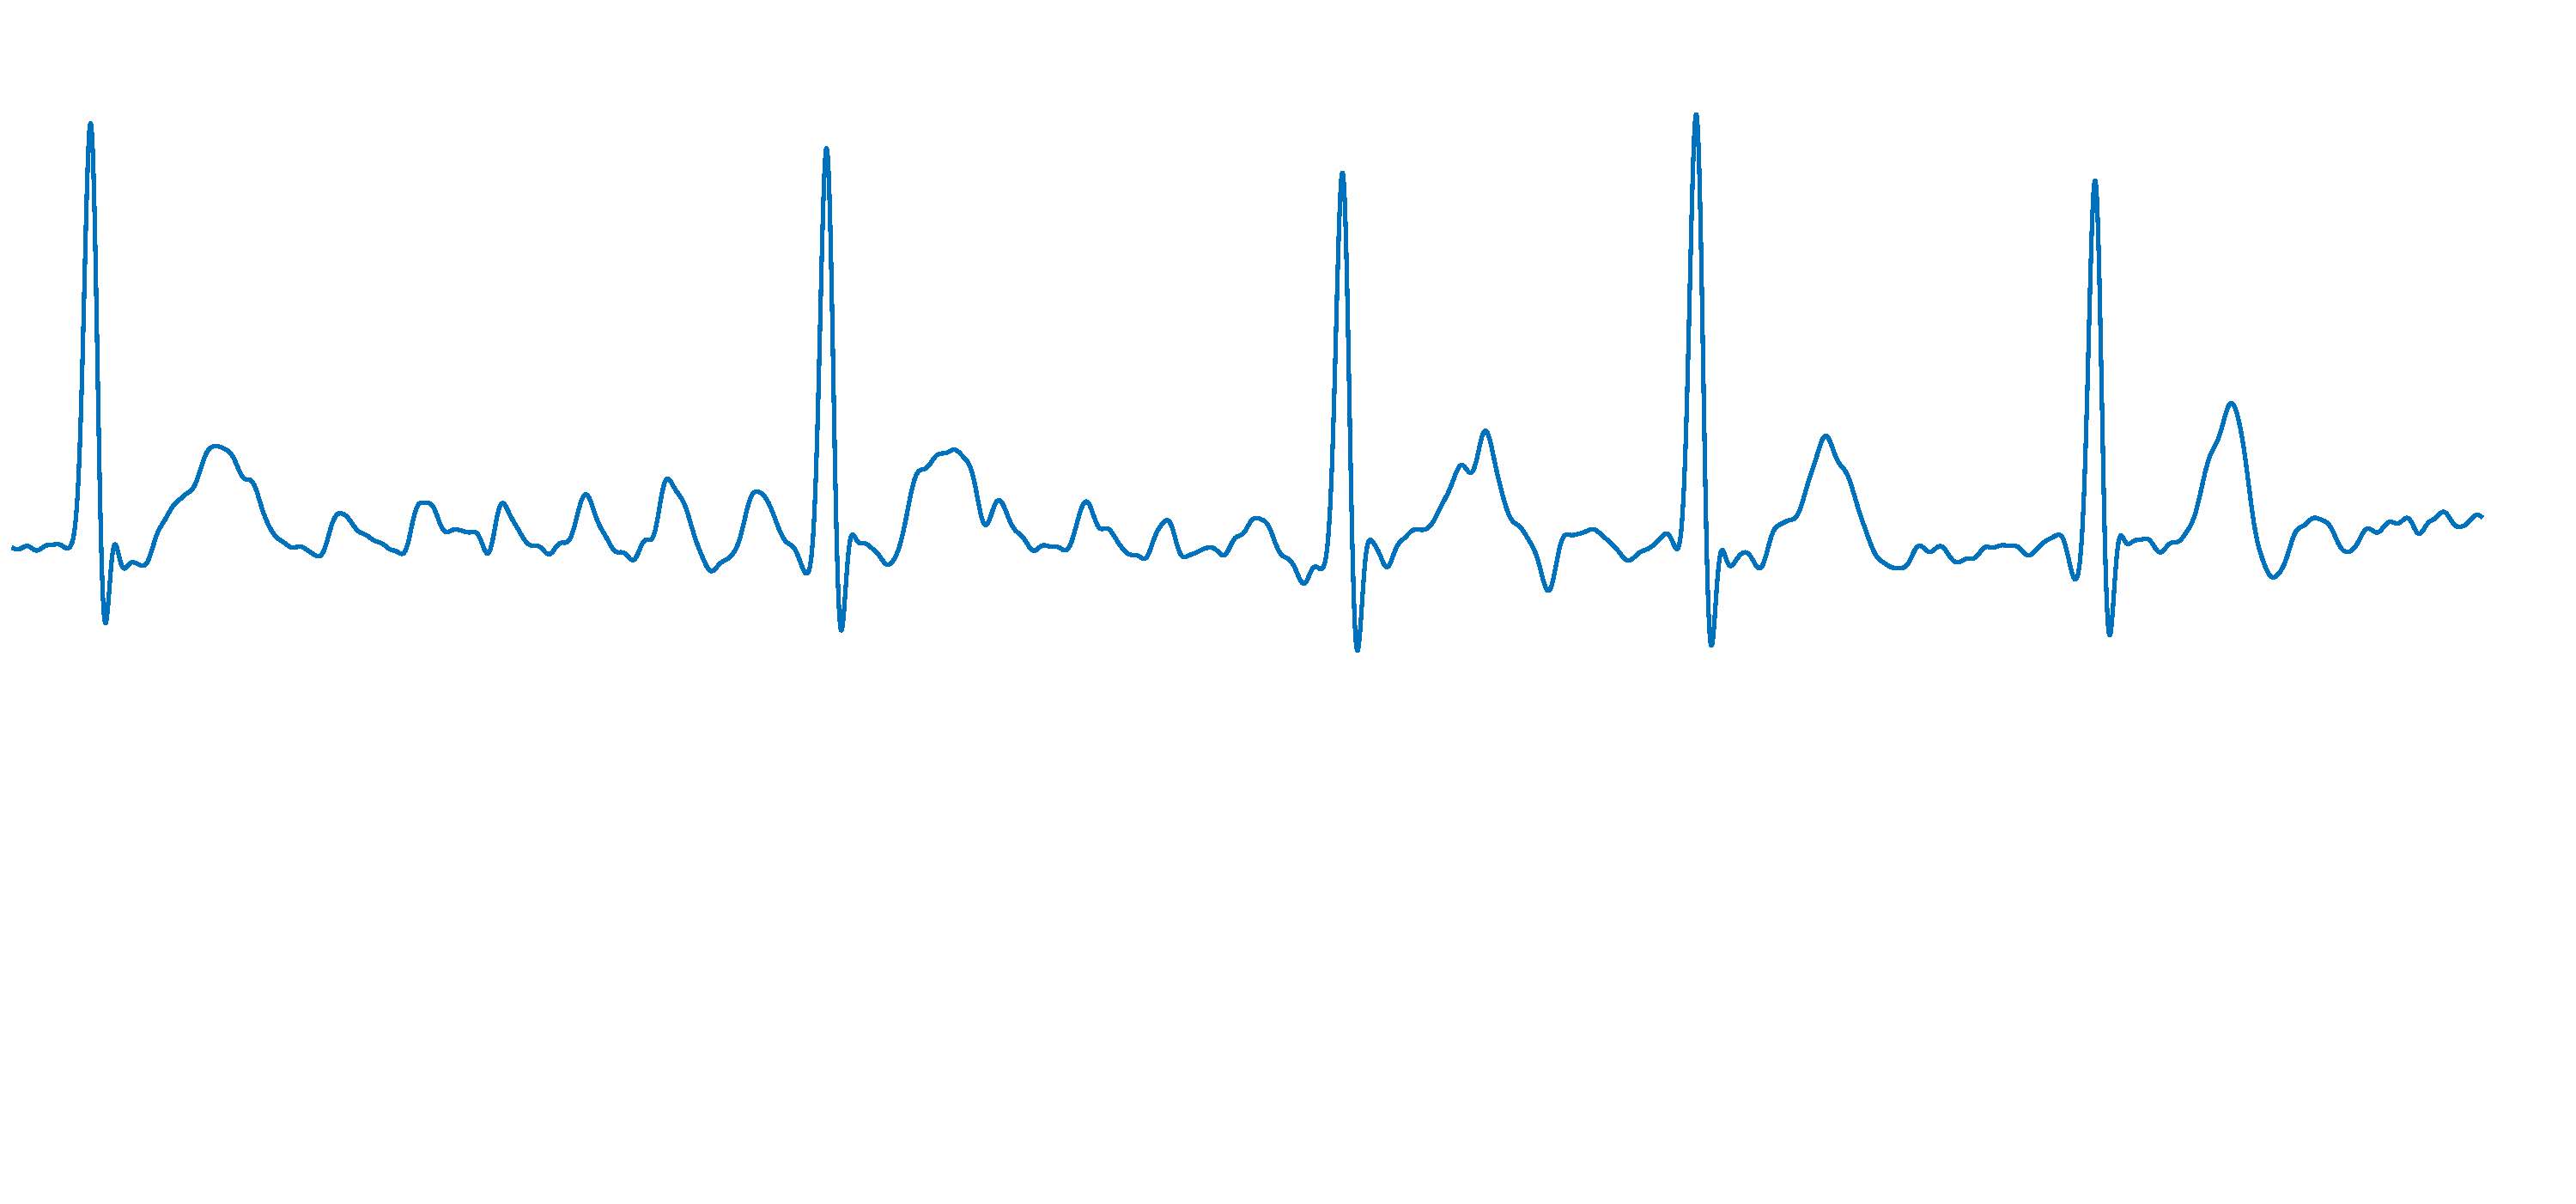
\includegraphics[scale=0.2]{fig/CinC2020/AF_ECG-eps-converted-to.pdf}
		\end{figure}
		\vspace{-0.8in}	
		\begin{itemize}
			\item The complex electrophysiological mechanisms underlying AF are not completely understood.
		\end{itemize}
	\end{frame}

	\begin{frame}{Step-wise Catheter Ablation (CA)}
		
		\begin{figure}[h]
			\centering
			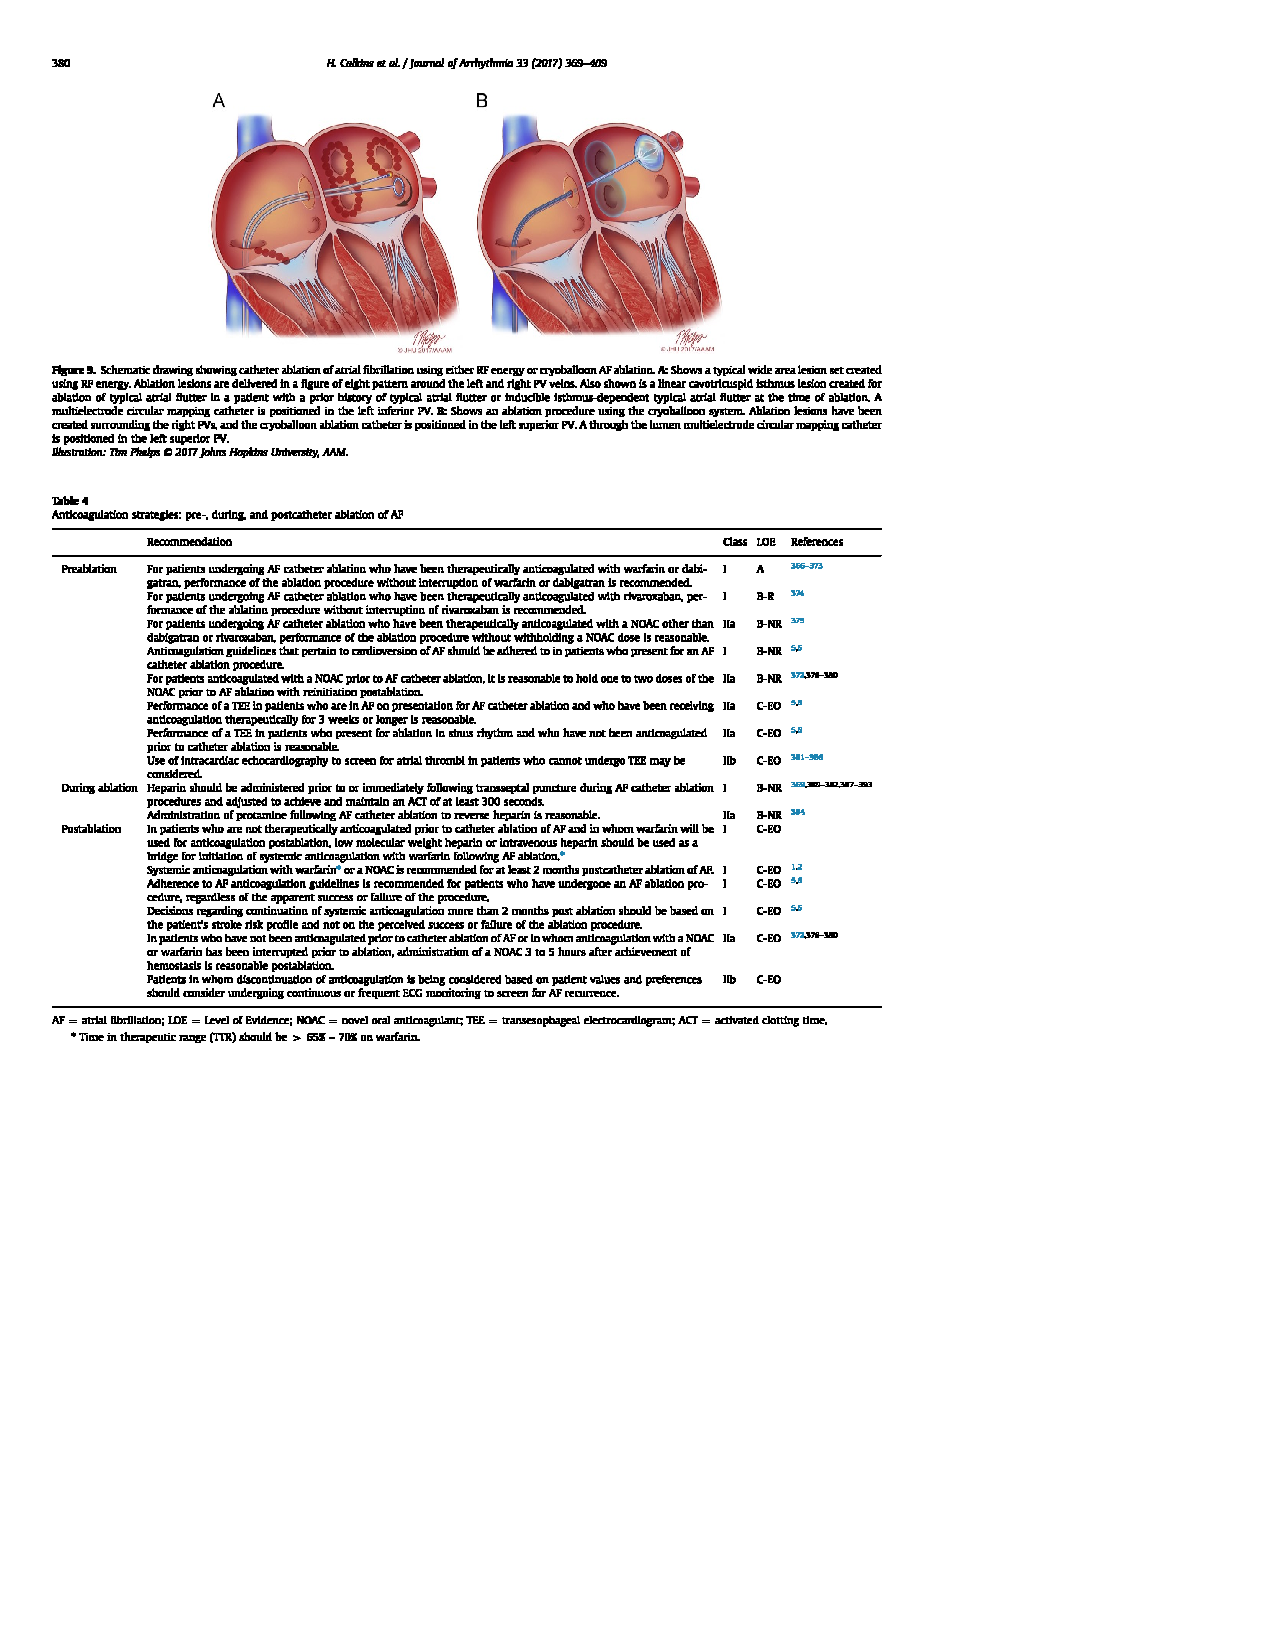
\includegraphics[scale=1.2,clip=true,trim={3.55cm 21.95cm 13.8cm 2.0cm}]{fig/CinC2020/CA_figure.pdf}
		\end{figure}
		\blfootnote{Figure from Tim Helps $^{\text{\tiny{\copyright}}}$ 2017 Johns Hopkins University, AAM}
		\vspace{-0.8cm}
		\begin{itemize}
			\item Noninvasive techniques to assess AF electrophysiological complexity can help guide step-wise CA in real time.
			\begin{itemize}
				\item Impact of pulmonary vein isolation (PVI) and other widely used techniques on atrial activity (AA) complexity.
			\end{itemize}
		\end{itemize}
	\end{frame}

	\begin{frame}{Matrix Approach}
	
		The ECG data matrix can be modeled as:
		\begin{equation}
			\textbf{Y} = \textbf{MS} \in \mathbb{R}^{K \times N} \; ,
		\end{equation}
		where ${\textbf{M}} \in {\mathbb{R}}^{K \times R}$ is a mixing matrix and $\textbf{S} \in {\mathbb{R}}^{R \times N}$ is the source matrix.	
		\vspace{-0.4cm}
		\begin{figure}[htb]
			\centering
			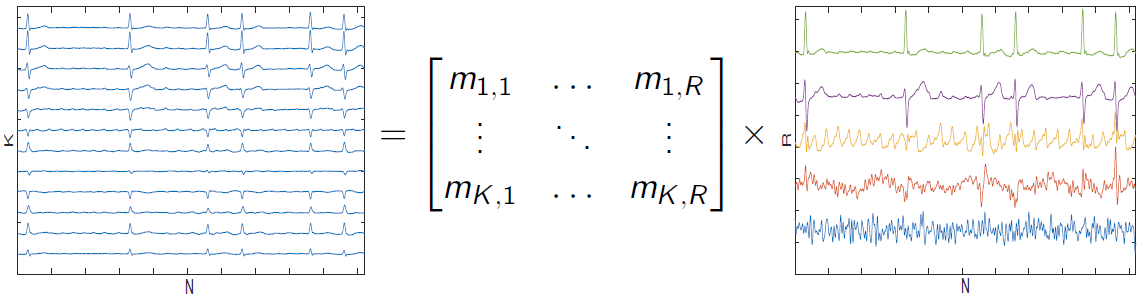
\includegraphics[scale=0.5]{fig/CinC2020/bss_fig.png}
		\end{figure}
	\end{frame}
		

%% ------------------------- Methods ------------------------------------------
\section{Methods}


	\begin{frame}{Low-rank Hankel Signal Model}
		
		\vspace{-0.5cm}
		\begin{block}{Model Framework}
			\begin{itemize}
				\item AA signal during AF can be represented by an all-pole model~(\ref{eq:hankel})
			\end{itemize}
			\begin{itemize}
				\item The Hankel matrix has a rank equal to the number of poles ($L$)
			\end{itemize}
		\end{block}
		\begin{columns}
			\begin{column}{0.3\textwidth}		
				% \vspace{2.5cm}
				\begin{align}
					s(n) = \sum_{\ell = 1}^{L} c_{\ell} z_{\ell}^{n} \label{eq:hankel} \\ \nonumber \\
					0\leq n \leq N-1 \nonumber
				\end{align}
			\end{column}
			\begin{column}{0.6\textwidth}
				\begin{figure}[htb]
					\vspace{-0.50cm}
					\centering
					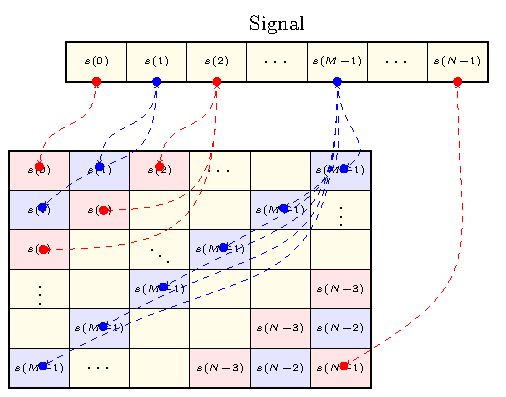
\includegraphics[scale=0.8]{fig/SBRT2021/tikz_mapHankel_NOTATION.pdf}
				\end{figure}
			\end{column}
		\end{columns}
	\end{frame}

	\begin{frame}{Vandermonde Decomposition}

		\begin{block}{Low-rank Hankel Structure}
			\begin{itemize}
				\item The sequence $s(n)$ with $N$ samples is mapped onto an $ (M\times M) $ Hankel matrix denoted ${\mathbf{H}}_s$
		    \end{itemize}
		\end{block}
	    
		\begin{itemize}
		    \item We assume $N$ is odd without loss of generality
		\end{itemize}
		
		\begin{equation}
		    M = \frac{N+1}{2}
		\end{equation}
	    
	    \begin{block}{Decompose a Low-rank Hankel Structure}
        	\begin{itemize}
        		\item The matrix ${\mathbf{H}}_s$ accepts Vandermonde decomposition~(\ref{eq:Hankel_Complete})
            \end{itemize}
        \end{block}
      \vspace{-10pt}
        \begin{equation}
            {\mathbf{H}}_s = {\mathbf{V}}_s \, {\mathbf{D}} \, {\mathbf{V}}_s^\intercal \label{eq:Hankel_Complete} 
        \end{equation}
	
	\end{frame}

	\begin{frame}{Model Framework}
    
        \begin{block}{Vandermonde Decomposition}
    		\begin{itemize}
       		    \item The poles of $s(n)$ are linked to the columns of matrix ${\mathbf{V}}_s$~(\ref{eq:Vandermonde})
    		\end{itemize}
        \end{block}

        \vspace{-10pt}
  
        \begin{equation}
            {\mathbf{V}}_s = \left[ \begin{array}{cccc}
            1 & 1 & \dots & 1 \\\\
            z_{1} & z_{2} & \dots & z_{L} \\\\
            \vdots & \vdots &  & \vdots \\\\
            z_{1}^{M-1} & z_{2}^{M-1} & \dots & z_{L}^{M-1}
            \end{array} \right] \in \mathbb{C}^{M \times L} \ , \label{eq:Vandermonde}
        \end{equation}
        
        \begin{itemize}
            \item As result of the Vandermonde decomposition, the Hankel matrix ${\mathbf{H}}_s$ has rank at most $\min\{L,M\}$\footnote{De Lathauwer, ``Blind separation of exponential polynomials and the decomposition of a tensor in rank-($L_{r}$,$L_{r}$,1) terms,'' \textit{SIAM J. Matrix Anal. Appl.}, 2011.}
        \end{itemize}

	\end{frame}	
    
    \begin{frame}{Model Framework}
    
        \begin{block}{Signal vs. Matrix Complexity}
            \begin{itemize}
                \item The more poles a given signal is composed of, the higher the rank of its Hankel matrix
                \item This observation underlies the use of $rank ({\mathbf{H}}_s)$ as a measure of signal complexity, where the rank $R$ is equal to $L$
            \end{itemize}
        \end{block}
        
        \vspace{10pt}
        
        \begin{itemize}
            \item To present $R$ equal to $L$, a Hankel matrix ${\mathbf{H}}_s$ with $L$ poles needs to map at least $N_{min}$ samples\footnote{Boley, ``A General Vandermonde Factorization of a {Hankel} Matrix,'' \textit{Int. Lin. Alg. Soc.(ILAS) Symp. on Fast Algorithms for Control, Signals and Image Processing}, 1997.}:
        \end{itemize}
        
        \begin{equation}
            N_{min} = 2L - 1 \label{eq:N_min-Samples}
        \end{equation}

    \end{frame}
    
    \begin{frame}{Vandermonde Matrix}
        
        \begin{block}{Poles Distance $(\Delta \omega)$ }
        	\begin{itemize}
        		\item When the distance between the poles decreases, the columns of ${\mathbf{V}}_s$ become closer to each other
        		\item It impacts on the Hankel matrix rank
            \end{itemize}
        \end{block}
        
        \begin{itemize}
            \item To illustrate this behavior, we assume two poles $z_1 = e^{j\omega_1}$ and $z_2 = e^{j\omega_2}$, and the corresponding Vandermonde vectors:
        \end{itemize}
        
        $$ {\bf{v}}_1 = [1, e^{\jmath \omega_{1}}, e^{\jmath 2 \omega_{1}}, \dots, e^{\jmath (M-1) \omega_{1}}]^\intercal$$ 
        $$ {\bf{v}}_2 = [1, e^{\jmath \omega_{2}}, e^{\jmath 2 \omega_{2}}, \dots, e^{\jmath (M-1) \omega_{2}}]^\intercal$$
        
        \begin{block}{Scalar Product}
    	    \begin{itemize}
    	        \item Assuming exponential identities and $\Delta \omega = (\omega_{2}-\omega_{1})$
    	    \end{itemize}
	    \end{block}
        
    \end{frame}
    
    \begin{frame}{Vandermonde Matrix and Poles Distance}

        The scalar product becomes:
        
        \begin{equation}
            \cos(\theta) = \frac{ {\bf{v}}_1 \cdot {\bf{v}}_2}{||{\bf{v}}_1||\,||{\bf{v}}_2||} = \frac{ \sin(M \frac{\Delta \omega}{2})}{ M \sin(\frac{\Delta \omega}{2})} \label{eq:scalar_product}
        \end{equation}
            
        When $\Delta \omega$ tends to zero for a fixed $M$, we have that:
        
        $$\lim_{\Delta \omega \to 0} \cos(\theta) = 1 $$
        
        \begin{block}{$\Delta \omega \to 0$}
    	    \begin{itemize}
                \item The columns becomes colinear
                \item The equivalent Hankel matrix rank ($R$) is equal to one, built from two damped exponentials, resulting in $R \neq L$
    	    \end{itemize}
	    \end{block}
	
	\end{frame}	

    \begin{frame}{Vandermonde Matrix and Poles Distance}
        
        However, we can deduce that increasing the value of $M$ used to build ${\mathbf{V}}_s$ may compensate for the poles proximity
        
        \begin{itemize}
            \item Replacing $M$ by its relation with $N$, we have that:
        \end{itemize}

        $$ \lim_{N \to \infty} \cos(\theta) = \frac{ 2\sin\left( (N+1) \Delta \omega \right)}{ (N+1) \sin\left(\frac{\Delta \omega}{2} \right)}$$
        
        $$ \lim_{N \to \infty} \cos(\theta) = 0 $$
        
        \begin{block}{$N \to \infty$}
    	    \begin{itemize}
                \item The scalar-product gets closer to zero, in such a way that colinearity between ${\bf{v}}_1$ and ${\bf{v}}_2$ is reduced
                \item Resulting in $R = L$, built from two damped exponentials
    	    \end{itemize}
	    \end{block}
	    
	\end{frame}
	
	\begin{frame}{Singular Value Decomposition}
		
		\begin{block}{Singular Value Decomposition}
			\begin{itemize}
				\item The Singular Value Decomposition (SVD) of ${\mathbf{X}} \in \mathbb{C}^{I\times J}$ is given by:
			\end{itemize}
		\end{block}
		\vspace{-10pt}
		\begin{equation}
			 {\mathbf{X}} = {\mathbf{U}} {\mathbf{\Sigma}} {\mathbf{V}}^H
		\end{equation}
		\vspace{-10pt}
		\begin{block}{Condition Number}
			\begin{itemize}
				\item A way to assess rank-deficiency is by the condition number ($\sigma$)
				\item It takes advantage of the relationship between singular values
			\end{itemize}
		\end{block}
		\vspace{-10pt}
		\begin{equation}
            \sigma = \frac{\lambda_{max}}{\lambda_{min}}
		\end{equation}
	\end{frame}

	\begin{frame}{Tensor Approach}
		
		\begin{itemize}
			\item The ECG data can be modeled as a 3rd-order tensor ${\mathcal{Y}}$ via row-Hankelization.
			\begin{itemize}
				\item Tensor decompositions factorize data as a sum of simpler tensors.
			\end{itemize}
		\end{itemize}
		\vspace{-0.7cm}
		\begin{figure}[htb]
			\centering
			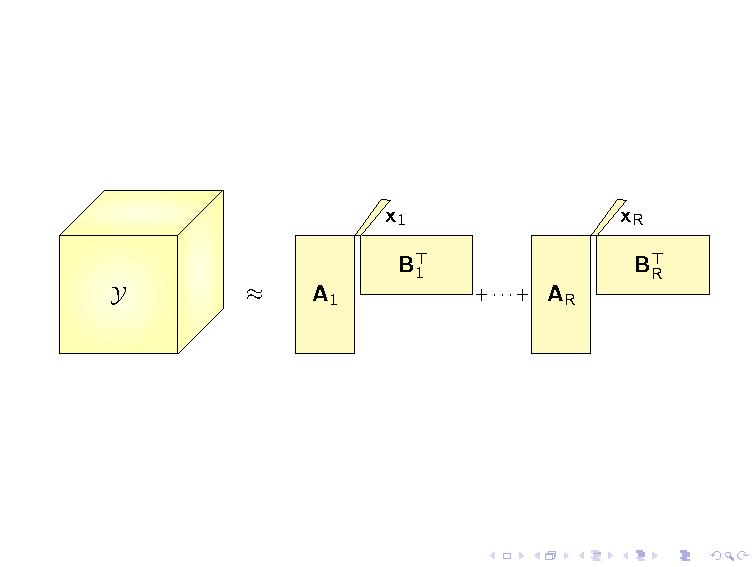
\includegraphics[scale=0.8,clip=true,trim={0.8cm 6.5cm 0.6cm 6.2cm}]{fig/CinC2020/tikz_BTDY.pdf}
		\end{figure}
		\vspace{2.3cm}
		\begin{itemize}
			\item Block Term Tensor Decomposition (BTD) based on Hankel structure\footnote{De Lathauwer, ``Blind separation of exponential polynomials and the decomposition of a tensor in rank-($L_{r}$,$L_{r}$,1) terms,'' \textit{SIAM J. Matrix Anal. Appl.}, 2011.}.
		\end{itemize}
	\end{frame}	

	\begin{frame}{Tensor Approach}
		
		\vspace{-3.5cm}
		\begin{itemize}
			\item Stack each Hankel matrix in the 3rd-mode of the tensor $\mathcal{Y}$.
		\end{itemize}
		
		\vspace{3.0cm}
		\begin{figure}[!ht]
			\centering
			\vspace{-3.5cm}
			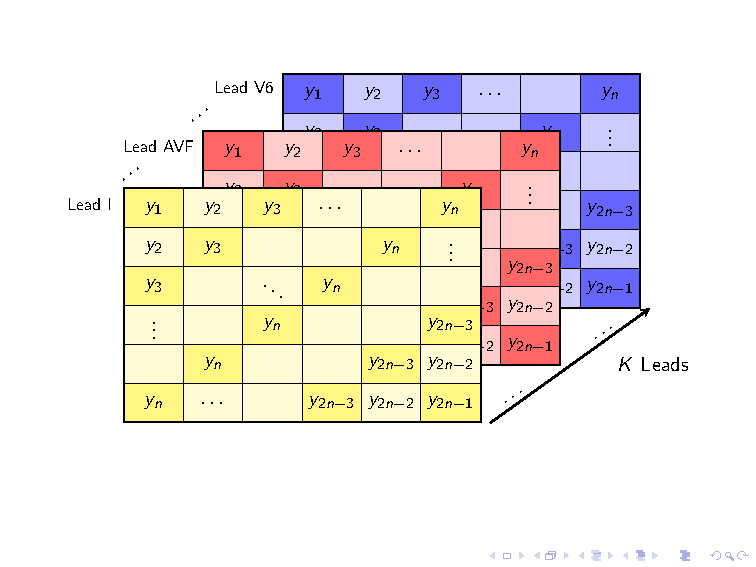
\includegraphics[scale=1.0,trim={1.0cm 8.5cm 1.0cm 7.3cm},clip=true]{fig/CinC2020/tikz_tensorHankel.pdf}
		\end{figure}
	\end{frame}

	\begin{frame}{BTD-Hankel Model}
		
		\vspace{-0.7cm}
		\begin{figure}[htb]
			\centering
			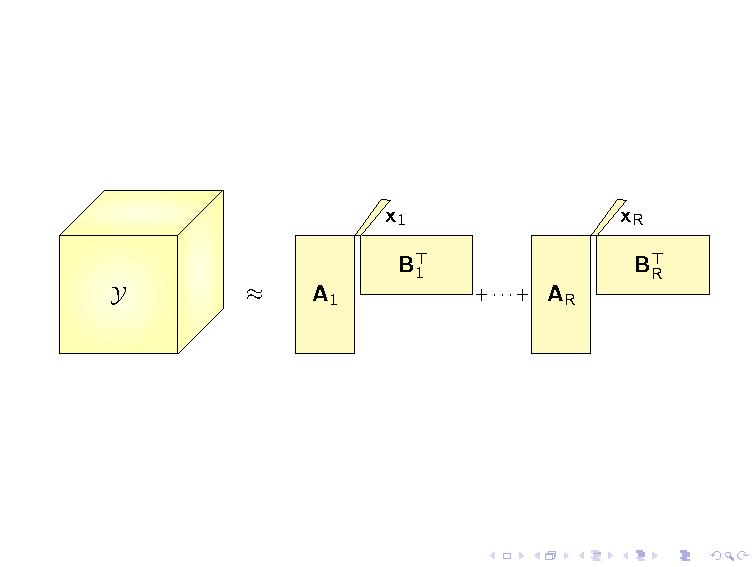
\includegraphics[scale=1.0,clip=true,trim={0.8cm 6.5cm 0.6cm 6.2cm}]{fig/CinC2020/tikz_BTDY.pdf}
		\end{figure}
		\vspace{2.8cm}
		\begin{block}{Challenge}			
				\begin{itemize}
					\item Parameter estimation
					\begin{itemize}
						\item $R$, $L$
					\end{itemize}
					\item Factor estimation
					\begin{itemize}
						\item $\textbf{A}$, $\textbf{B}$, $\textbf{X}$
					\end{itemize}
				\end{itemize}
		\end{block}
	\end{frame}

	\begin{frame}{Constrained Alternating Group Lasso}
		
		\begin{block}{Classical BTD Approach}
			\begin{itemize}
				\item Fixed structure minimizing $f(\textbf{A}, \textbf{B}, \textbf{X})$ with prior knowledge of $(R,L)$
			\end{itemize}
		\end{block}
		\begin{equation}
			f(\textbf{A}, \textbf{B}, \textbf{X}) \triangleq
			 \Big\| {\mathcal{Y}} - \textstyle \sum_{r = 1}^{R} \left( \textbf{A}_r \textbf{B}_r^{\top} \right) \circ \textbf{x}_r  \Big\|_F^2
		\end{equation}
		\begin{block}{Constrained Alternating Group Lasso (CAGL) Approach}
			\begin{itemize}
				\item Non-fixed structure minimizing $F(\textbf{A},\textbf{B},\textbf{X})$ ensuring the Hankel structure
				\item Penalization term ($\gamma$) and $g({\textbf{A}, \textbf{B}, \textbf{X}})$ limiting the multilinear ranks and number of blocks
				\item Allows simultaneous estimation of $(R,L)$ and model factors
			\end{itemize}
		\end{block}
		\begin{equation}
				  F({\textbf{A}, \textbf{B}, \textbf{X}})
				 \triangleq  
				 f({\textbf{A}, \textbf{B}, \textbf{X}}) + \gamma \, g({\textbf{A}, \textbf{B}, \textbf{X}})
		\end{equation}
	\end{frame}
	
	\begin{frame}{AF Complexity Index}
		
		\begin{block}{Signal Complexity}
			The more poles the signal contains, the more complex it can be considered
		\end{block}
		
		\begin{itemize}
			\item The complexity index proposed in this work is based on the number of poles $L$ contained in a signal. 
			\item The Hankel matrix rank is equal to number of poles $L$.
		\end{itemize}

	\end{frame}

	
%% ------------------------- Experimental Results -----------------------------
\section{Results: Hankel Signal Model }
	
	\begin{frame}{Condition Number}

	    \begin{block}{Experiment Framework}
        	\begin{itemize}
        	    \item We build a Vandermonde matrix from two vectors to illustrate how a small $\Delta \omega$ hamper the construction of a full-rank matrix
        	    \item How it impacts the condition number
        	\end{itemize}
		\end{block}

        \begin{itemize}
            \item Assuming two vectors ${\bf{v}}_1$ and ${\bf{v}}_2$ as the columns of the Vandermonde matrix ${\mathbf{V}}_s$, with $\omega_1 = 0$, and $\omega_2 = \Delta \omega$, \textit{i.e.}:
        \end{itemize}
		
		\vspace{-10pt}

		$$ {\bf{v}}_1=[1, 1, 1, \dots, 1]^\intercal $$
		
		\vspace{-10pt}
		
		$$ {\bf{v}}_2 = [1, e^{\jmath\Delta\omega}, e^{\jmath2\Delta\omega}, \dots, e^{\jmath(M-1)\Delta\omega}]^\intercal $$
		
		\begin{block}{Numerical Assessment}
		    \begin{itemize}
			    \item Compute the SVD$({\mathbf{H}}_s)$ for 10 different values of $N$, rounding logarithmically spaced values in the interval $[10^{1},10^{2}]$, and considering 7 different values of $\Delta \omega$.
		\end{itemize}
		\end{block}

	\end{frame}

	\begin{frame}{Condition Number}
        
        \vspace{-20pt}

        \begin{figure}[!ht]
			\centering
			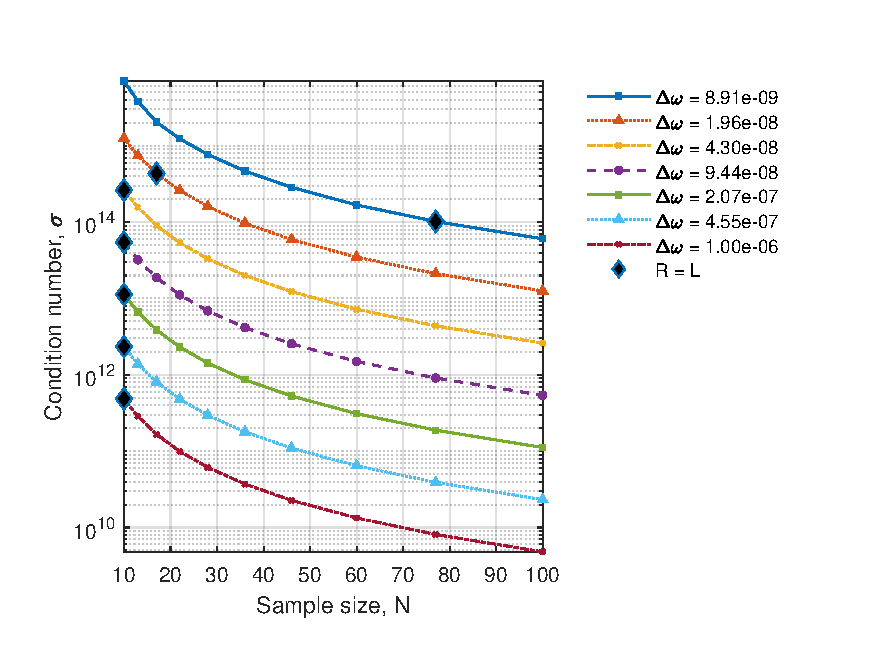
\includegraphics[scale=0.80]{fig/SBRT2021/eigen_hankel-conditionNumber3-2021-05-15.pdf}
		\end{figure}

	\end{frame}
	
	\begin{frame}{Condition Number}
        
        \begin{block}{Numerical Results}
            \begin{itemize}
        	    \item The distances between poles are so small that even increasing the number of samples, $\sigma$ keeps very high
        	    \item This behavior affects rank computation and may prevent us to obtain $R = L$
        	    \item The value of $\sigma$ decreases as we increase the number of samples to the columns, which compensates for the poles proximity as expected from our previous analysis
        	\end{itemize}
        \end{block}
	        
	\end{frame}

	\begin{frame}{Sample Size for a Full-Rank Hankel Matrix}
	    
        \begin{block}{Experiment Framework}
        	\begin{itemize}
        	    \item We test various distances between poles to assess the minimum amount of samples necessary to obtain the Hankel matrix rank equal to the number of poles contained in the signal
    	    \end{itemize}
    	\end{block}

	   We build ${\mathbf{H}}_s$ from 100 samples for each $s(n)$, where:
	   
	   \begin{itemize}
	        \item $L$ is in the [2,8] interval;
	        \item $z_l$ represent equispaced poles;
	        \item $\Delta \omega$ takes 100 logarithmically spaced values in the $[10^{-4},10^{-1}]$ interval;
	        \item We assume $c_l = 1 \ , l = 1, 2, \dots, L$ for simplicity, but without loss of generality.
	   \end{itemize}

	\end{frame}
	
	\begin{frame}{Sample Size for a Full-Rank Hankel Matrix}
		
		\begin{block}{Numerical Assessment}
		    \begin{itemize}
        	    \item To compare the numerical and theoretical results, we use a windowed version of $s(n)$ with $N \leq 100$ samples to build its equivalent Hankel structure
        	    \item The number of samples used in window $N$ is a positive integer value between 2 and 100. 
        	    \item Summarized as follows: for each value of $L$ in the set of positive integers, we vary $\Delta \omega$ from very close poles gradually moving them away from each other at each iteration, noting the value of $N$ for $R = L$.
    		\end{itemize}
		\end{block}
		
	    
	\end{frame}
	
	\begin{frame}{Sample Size for a Full-Rank Hankel Matrix}
        
        \vspace{-20pt}

        \begin{figure}[!ht]
			\centering
			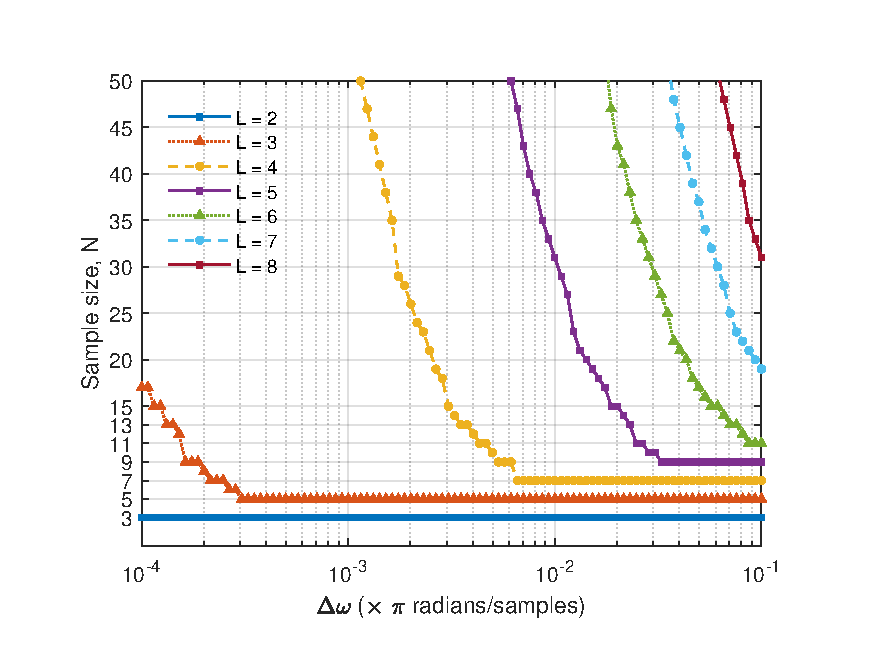
\includegraphics[scale=0.75]{fig/SBRT2021/poles_proximity-PoleDistance_vs_Samples-2021-05-14.pdf}
		\end{figure}

	\end{frame}
	
	\begin{frame}{Sample Size for a Full-Rank Hankel Matrix}
        
        \begin{block}{Numerical Results}
            \begin{itemize}
                \item The experiment shows that the theoretical values are different from those obtained empirically (One would expect plots with horizontal lines at $2L - 1$ regardless of $\Delta \omega$)
                \item When the distance gets smaller, the number of samples $N$ necessary in the windowed signal to build ${\mathbf{H}}_s$ with $R=L$ increases
                \item This outcome reinforces the hypothesis that the increase of $N$ may compensate for the distance between poles to obtain $R=L$ as anticipated
        	\end{itemize}
        \end{block}

	\end{frame}

	\begin{frame}{Noisy Scenario and SNR Threshold}

	    \begin{block}{Experiment Framework}
        	\begin{itemize}
        	    \item We reproduce the previous setup, but signals are analyzed with various SNR values with a fixed distance between poles.
        	\end{itemize}
		\end{block}
        
        Considering a scenario with additive white Gaussian noise (AWGN):
        
		\vspace{-10pt}

		$$ y(n) = s(n) + \beta(n) $$
		
		\begin{itemize}
		    \item The mapped signal $y(n)$ is a version of $s(n)$ affected by the AWGN term $\beta(n)$, and with $\Delta \omega = 0.05$. 
		\end{itemize}
		
		\begin{block}{Numerical Assessment}
		    \begin{itemize}
                \item We perform 100 Monte Carlo runs, varying the noise for each realization.
			    \item For each value of $L$ in the set of positive integers [2,8], we vary SNR values along the [250,320] interval in 10 dB steps, at each iteration, noting the value of $N$ for $R = L$.
		    \end{itemize}
		\end{block}
		
	\end{frame}
	
	\begin{frame}{Noisy Scenario and SNR Threshold}
        
        \vspace{-20pt}

        \begin{figure}[!ht]
			\centering
			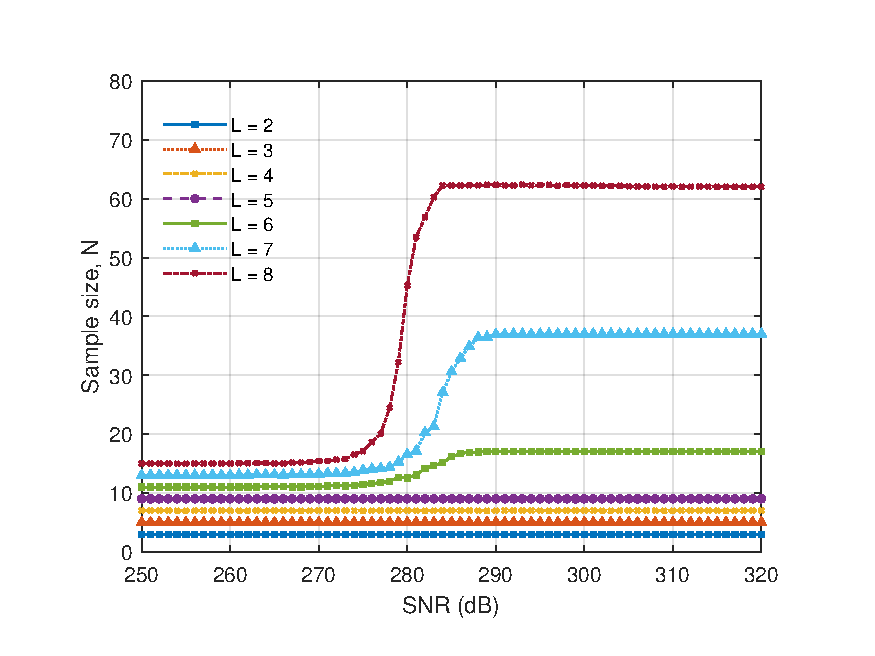
\includegraphics[scale=0.75]{fig/SBRT2021/SNR_proximity-MonteCarlo-with-100runs--2021-05-15.pdf}
		\end{figure}
		
	\end{frame}

	\begin{frame}{Noisy Scenario and SNR Threshold}
        
        \begin{block}{Numerical Results}
            \begin{itemize}
                \item The experiment shows that for values of SNR less than 270 dB, in general the most commonly encountered in real problems, the theoretical result is respected (Expected plots with horizontal lines at $2L - 1$)
                \item However, for values greater than 270 dB, the theoretical values are once again different from those obtained empirically, but $N$ starts to increase.
                \item When the SNR gets greater, the number of samples $N$ necessary in the windowed signal to build ${\mathbf{H}}_s$ with $R=L$ increases
        	\end{itemize}
        \end{block}

	\end{frame}
	

%% ------------------------- Experimental Results -----------------------------
\section{Results: Real ECG Scenario}

	\begin{frame}{Atrial Source Classification}
			
			\begin{block}{Challenge}
				After performing CAGL, the automated AA source classification is still a problem
			\end{block}
			
			\begin{itemize}
				\item Spectral concentration (SC), dominant frequency (DF), kurtosis and visual inspection to evaluate AA extraction\footnote{De Oliveira and Zarzoso, ``Source analysis and selection using block term decomposition in atrial fibrillation'', in \textit{Proc. LVA/ICA}, 2018.}.
			\end{itemize}
	\end{frame}	

	\begin{frame}{AA Source Estimation}
		
		\vspace{-1.5cm}
		\begin{figure}[!ht]
			\centering
			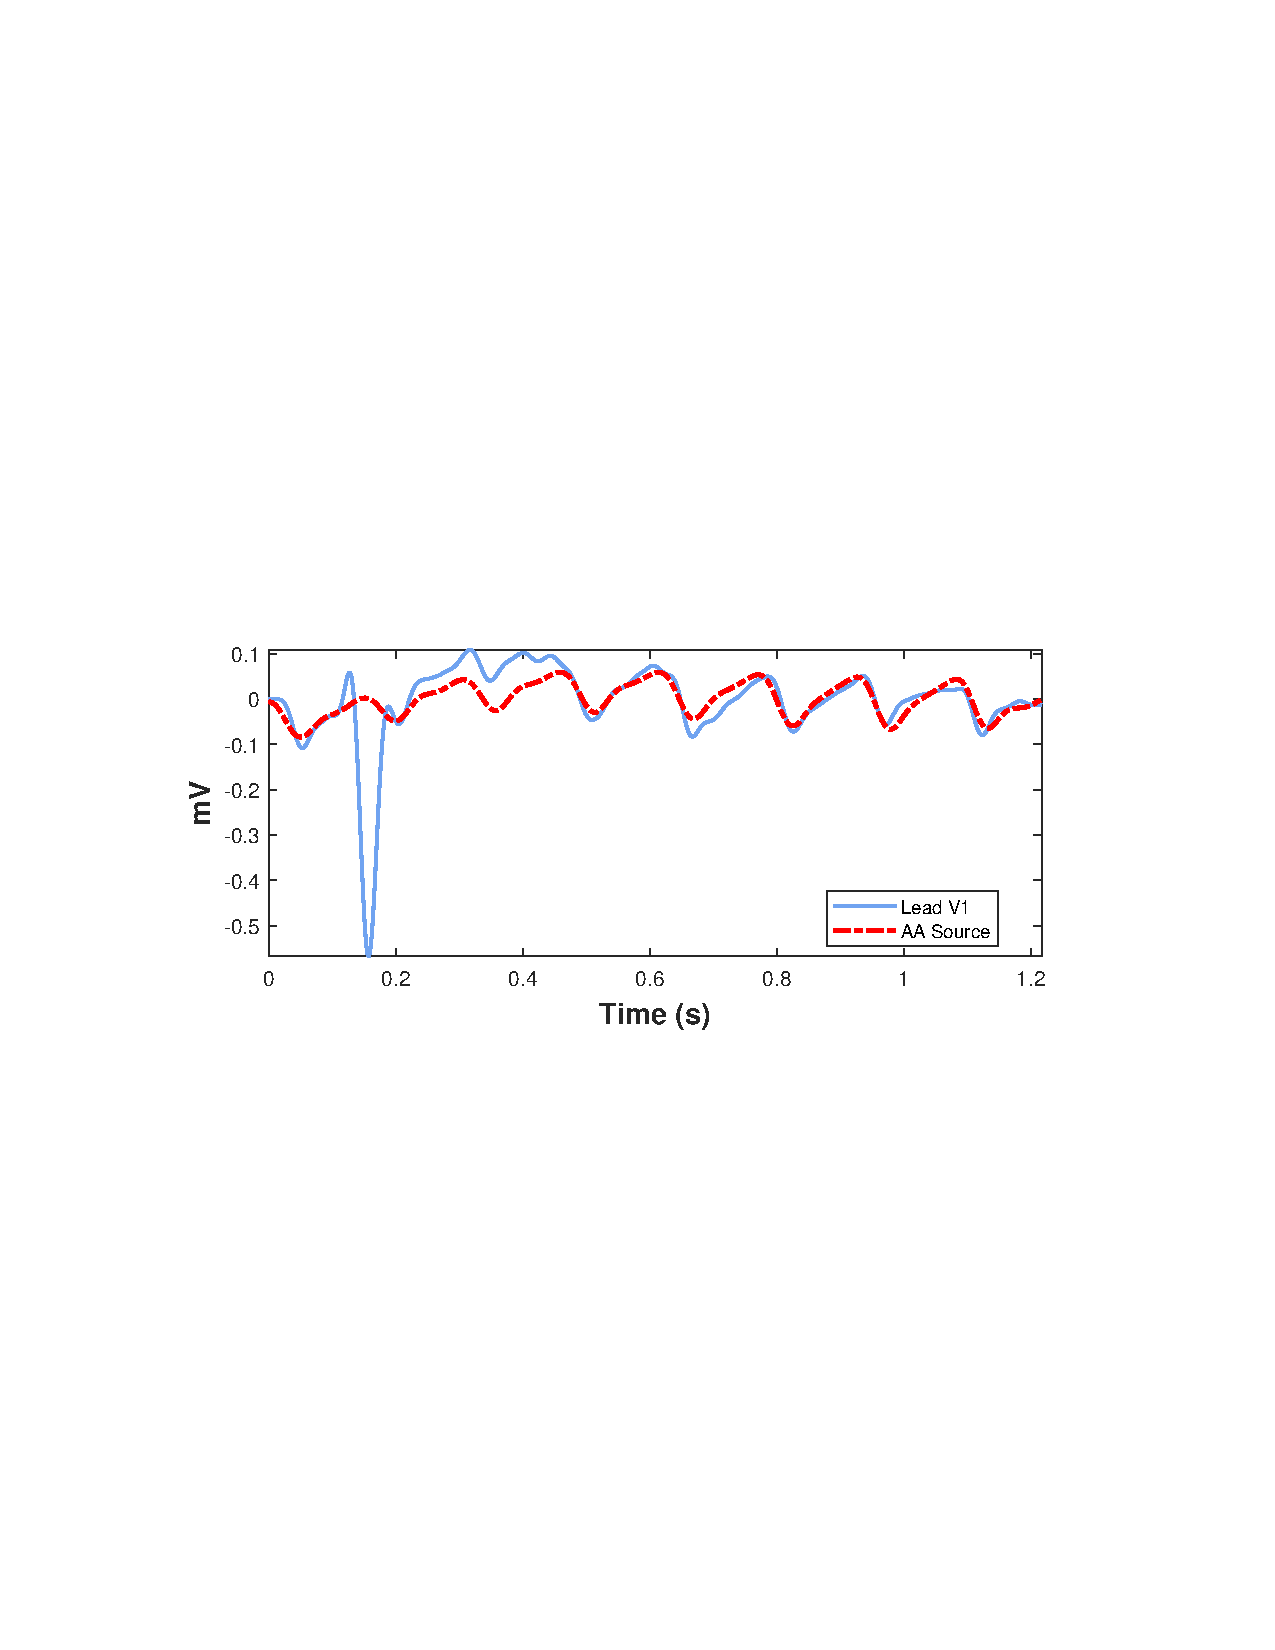
\includegraphics[scale=0.75,trim={3.0cm 8.5cm 3.0cm 8.5cm},clip=true]{fig/CinC2020/example_Source.pdf}
		\end{figure}
		\vspace{-2.0cm}
		
		\begin{itemize}
			\item SC $=$ 74.3\%
			\item DF $=$ 6.4 Hz
			\item Kurtosis $=$ 177.0
			\item AA Hankel Matrix Rank $=$ 33
		\end{itemize}
		
	\end{frame}
	
	\begin{frame}{Database and Experimental Setup} 
			
		\begin{block}{Database}
			\begin{itemize}
				\item 20 patients suffering from persistent AF
				\item 59 ECG segments from 0.72 to 1.42 seconds
			\end{itemize}
			
			\begin{center}
				Cardiology Department of Princess Grace Hospital Center, Monaco
			\end{center}					
		\end{block}	
		
		\begin{itemize}
			\item Hankel-based BTD was implemented using CAGL.
		\end{itemize}
	\end{frame}

	\begin{frame}{Impact of CA step on AA complexity}
		
		\vspace{-0.5cm}
		\begin{figure}[h]
			\centering
			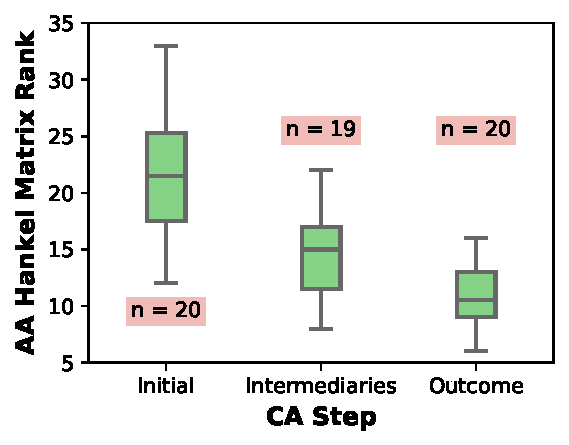
\includegraphics[scale=0.9]{fig/CinC2020/boxplot_complexity.pdf}
		\end{figure}
		\vspace{-0.5cm}
		\begin{itemize}
			\item 20 patients undergoing various CA steps
			\item 59 ECG segments (1.06 $\pm$ 0.2 s)
		\end{itemize}
	\end{frame}

	\begin{frame}{Impact of PVI on AA complexity}

		\vspace{-0.5cm}
		\begin{figure}[h]
			\centering
			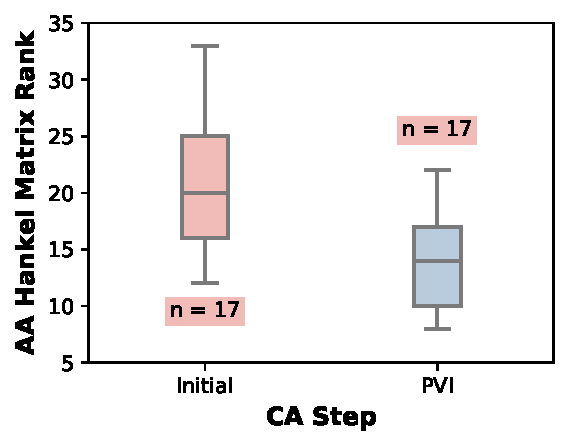
\includegraphics[scale=0.9]{fig/CinC2020/boxplot_PVI.pdf}
		\end{figure}
		\vspace{-0.5cm}
		\begin{itemize}
			\item 17 patients undergoing PVI
			\item 34 ECG segments
		\end{itemize}
	\end{frame}

	\begin{frame}{AF Recurrence vs. Complexity Before CA} 
		
		\vspace{-0.3cm}
		\begin{figure}[h]
			\centering
			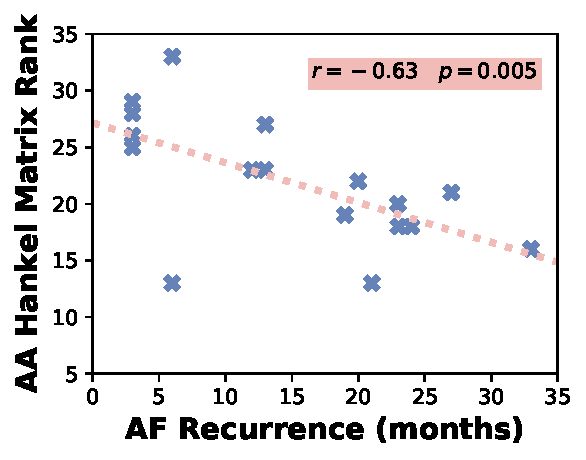
\includegraphics[scale=0.7]{fig/CinC2020/rank_LR.pdf}
		\end{figure}
		\vspace{-0.5cm}
		\begin{block}{Relationship}
			A significant Pearson correlation between AF recurrence and the proposed index
			\begin{itemize}
				\item 18 patients with complete follow-up information
			\end{itemize}
		\end{block}	
	\end{frame}

%% ------------------------- Conclusion ---------------------------------------
\section{Conclusions}

	\begin{frame}{Conclusions} 
		
		% \begin{block}{Contributions}
			\begin{itemize}
				\item Numerical features of Hankel matrices associated with complex exponential signal models
				\item To assure a full rank matrix, a minimum distance between poles is required or the number of mapped samples must increase to compensate for poles proximity
				\item With a realistic noise level, the Hankel matrix was always full rank, since the noise acts to balance the linear independence between the columns in the associated Vandermonde matrix.
				\item Jointly extract the AA signal and measure AF complexity via tensor decomposition
				\item Very short ECG recordings (1.06 $\pm$ 0.20 s)
				\item Validation in 20 patients undergoing CA
				\begin{itemize}
					\item Expected decreasing AF complexity throughout CA steps
					\item Significant correlation with AF recurrence after CA
				\end{itemize}
			\end{itemize}
		% \end{block}
		
		
	\end{frame}


	\begin{frame}{Further Work} 

	\begin{block}{Clinical Impact}
			\begin{itemize}
				\item A potential tool to help guide CA in real time
			\end{itemize}
	\end{block}

	\vspace{1cm}
	% \begin{block}{}
		\begin{itemize}
			\item Performing the experiments for larger matrices, in order to provide more relevant statistical information.
			\item Explore the BTD context, since it performs the separation of the noise and the low-rank Hankel signal model in different blocks and it could fall within the noiseless scenario.
			\item Increase number of patients in the database
			\item Compare the proposed index with other state-of-the-art indices
			% \item Automated source classification.
		\end{itemize}
	% \end{block}
	
	\end{frame}


\end{document}